One major constraint of future High-Performance Computing (HPC) systems is their power
consumption.  Agencies have set strict targets for building an exascale machine --- e.g.,
the US Department of Energy has set the limit to 20MW~\cite{Ashby2010} --- while others,
like the European Union, are investing in novel approaches leveraging mobile technologies
to build low-power HPC infrastructures~\cite{Rajovic2013}.  The resulting need for
reducing hardware power consumption has started to force computer architects and vendors
to include power capping capabilities in their hardware designs.  This allows applications
to more efficiently exploit their entire power envelope of a system, while  guarding the
system against intermediate power spikes. Prior work has shown that this can lead to
significant performance benefits ~\cite{patki:2013:eho:2464996.2465009,conductor2015}.

Manufacturing variability, however, causes  processors and DRAM memories to react
inhomogeneously to power constraints enforced by the system. While already present in
current systems, such variability has so far been hidden by varying power consumption to
achieve homogeneous performance.  In fact, existing studies show a variation of up to 10\%
in power consumption to deliver the same performance~\cite{Rountree2012}. With the ability
to vary power removed by imposing a particular power limit, this variation becomes visible
in realized performance ~\cite{Inadomi:2015:AMI:2807591.2807638}.  Further, this uneven
distribution of delivered performance is specific to each single hardware component, since
two nominally identical processors can suffer from different degrees of manufacturing
issues.  From the HPC applications perspective, this can cause load imbalances, even if
the workload is perfectly balanced, resulting in significantly degraded performance.

To make this problem even worse, since such degradations are hardware specific, it is not
possible to design static or hardware agnostic techniques to mitigate this induced new
type of load imbalance. In this Chapter we propose an application agnostic, runtime-based
approach to mitigate the effects of manufacturing variability on NUMA nodes.  Our approach
tries different configurations of power distribution and number of active cores on each
socket on a NUMA node, while monitoring the performance of the application periodically,
for small fraction of the overall execution.  This way, the different configurations are
rated for their performance and the best one chosen for the rest of the execution.

 \begin{figure}[ht]
				\centering
        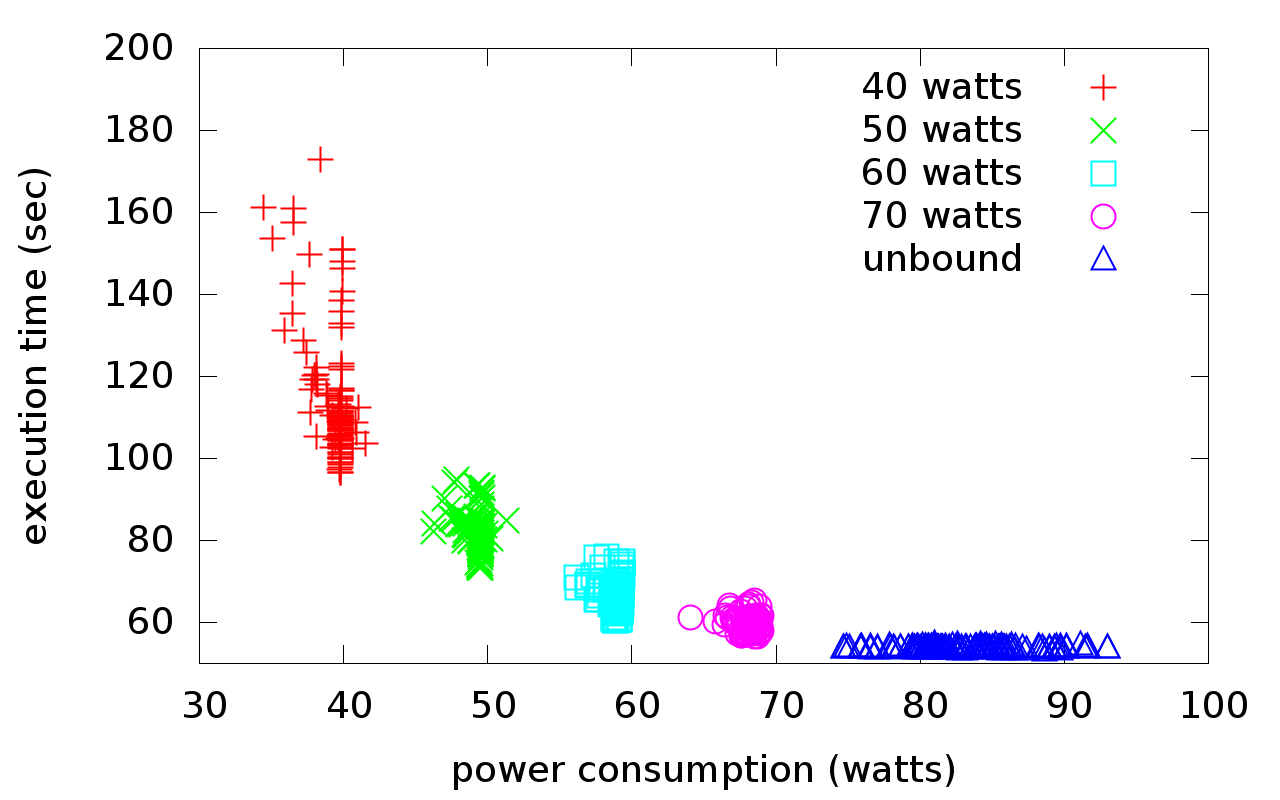
\includegraphics[width=\columnwidth]{background/figures/freqmine_power2perf_per_socket}
        \caption{Performance obtained when the \texttt{freqmine} application is run on 64 different 12-core Intel Xeon E5-2695v2 sockets under different power budgets.}
        \label{fig:socket_perf_variation}%
\vspace{.5cm}
\end{figure}

  
